\documentclass[11pt, oneside, fleqn]{article}
\usepackage[top=1.25in, bottom=1.25in]{geometry}
\geometry{letterpaper}
\usepackage[parfill]{parskip}			% Activate to begin paragraphs with an empty line rather than an indent

\usepackage{amssymb}
\usepackage{amsmath}
\usepackage{graphicx}

\pagestyle{empty}	% No page number in the footer.
\begin{document}
  \begin{center}
  \LARGE{Exploring Carl de Marcken's Word Segmentation}\\[0.5em]
  \large{Brian Hempel and Yuxi Chen}\\[0.5em]
  \large{June 8, 2016}\\[0.5em]
  \end{center}

  \vspace{1em}

  \section{Introduction}

  Carl de Marcken, in his PhD thesis ``Unsupervised Language Acquisition'', attempted to learn words given a large corpus of sentences devoid of all spaces and punctuation, similar to how children learn words from no prior information. In his thesis, de Markcen models learning by searching for a grammar that minimizes the combined description length of the input and the grammar together. Both sentences and words in the grammar are represented by composing smaller words. His method iteratively adds and deletes new grammar entries based on the goal. The hope is that patterns in the final grammar reflect the underlying mechanisms and parameters of the language that generated the input.
  
  \section{What We Did}

  We focus on re-implementing the learning algorithm of Carl de Marcken's PhD thesis. The general idea is to start with the simplest grammar, then iteratively refine the entries of the grammar to reduce the description length until convergence. 
  
  In the first part of each iteration, stochastic properties are optimized assuming a fixed linguistic structure in the grammar. The expectation-maximization algorithm is used to approach a locally optimal set of probabilities for the word in the lexicon.
 
  After optimizing the stochastic properties, the algorithm adds words to the grammar. Candidate words are composed of pairs of existing words that occur together at least twice in the soft counts calculated over the lexicon and the corpus. An estimation is made of the change in description length presuming the word is added and its parts possibly deleted. If the description length will decrease, the pair is added as a new word in the grammar.

  After another round of stochastic optimization, a similar estimation is used to delete words from the grammar. 
  
  We run the algorithm for 15 iterations. De Marcken discussed convergence criteria in his thesis, but chose to simply run his algorithm for 15 iterations for simplicity and to avoid the algorithm entering a loop where the same words are added and deleted repeatedly on successive iterations due to inaccuracy in the estimates used to determine when a word is added and deleted.
  
  \subsection{Implementation Notes}
  
  For the forward-backward stochastic optimization step, we calculate probabilities using log probabilities to avoid floating point underflow.

  On the input corpus, we downcase the input and delete all non-alphanumeric characters, including whitespace. In order to speed up processing, we use PyPy instead of CPython. With PyPy and several internal optimizations, a full run on the entire Brown Corpus takes roughly five hours.
  
  Our tool produces several output files:

  \begin{itemize}
    \item The found lexicon, as flat words (one word per line, most common word first).
    \item The true lexicon, as flat words (one word per line, most common word first).
    \item The found segmentation of the corpus, as flat words.
    \item The found segmentation of the corpus, with words given by their full nested representation.
    \item The true segmentation of the corpus, as flat words. 
  \end{itemize}

	We consider hyphens and whitespace as true word separators in the original corpus. A glance at the Brown corpus suggested to us that most hyphenated utterances should be considered multiple words.

  \subsection{Evaluation Criteria}

	In the algorithm, lexicon entries are a hierarchy of other lexicon entries. To judge performance, de Marcken compared these hierarchies with the true segmentation. De Marcken's recall rate is the proportion of the words in the true segmentation that also appear at some level of the algorithm's hierarchical parse of the input. The crossing-brackets rate (analogous to precision) measures a concept called crossing-bracket violations. A word in the true segmentation is considered a crossing bracket violation if a word in any level of the found hierarchical representation starts/ends in the true word but also crosses over into a neighboring word.
    
    With these metrics, de Marcken claims a recall of 90.5\% and a crossing-brackets rate of 1.7\%, which makes his work sound highly performant.

	The problem is that we don't know which level in the hierarchy has the correct word. Instead, we consider only the top level of hierarchy as the found word for segmentation.

	We evaluate the performance of the algorithm and our experiments below by measuring the precision and recall for three different comparisons against the true segmentation:
	
	\begin{enumerate}
		\item We compare the set of word break locations found in the corpus to the the true word break locations.
		\item We compare the words in the found segmentation to the true words at each corpus location.
		\item We compare the set of words in the found lexicon to the set of words in the true lexicon.
	\end{enumerate}

  \section*{Experiments}
  
  We made several kinds of modifications to the baseline algorithm to see how they change segmentation performance. All tests were performed on the Brown Corpus, which contains 44,195 unique words across 14,342 sentences.

  \subsection{Flat Words in Lexicon}
  
  De Marcken uses a nested representation for all words in the lexicon; that is, words are composed of other words. We tend not to think of words as being made up of smaller words, so what if we instead require all words in the lexicon to be represented by sequences of single characters?

  \subsection{Flat Words in Lexicon, Separate Lexicon Probability Model}

	De Marcken's baseline algorithm uses the same probability model for words in the lexicon and words in the sentences. This method breaks down pretty heavily in the naive ``Flat Words in Lexicon'' model above. Single characters are overrepresented for parsing the corpus, and words are overrepresented for parsing the lexicon.
	
	Instead, in this experiment we keep a character probability model specifically for representing the words in our lexicon. The word probabilities for the corpus are kept separately.

  \subsection{Flat Words in Lexicon, O(1) Lexicon Probability Model}

	Life experience suggests to us that real words have structure. The zero-order probability model of the previous experiment cannot capture structure. In this experiment we use a first order probability model for representing the words in our lexicon: the probability for each character is conditioned based on the prior character. Thus, character pairs uncommon to words are penalized.
	
	\textit{An implementation detail:} When character pairs probabilities are recalculated, we can't let any probability be 0; otherwise we won't be able to use that character. To avoid this, when counting characters instead of counting from 0 each character count is instead initialized to the 0-order probability of the character (a number between 0 and 1) and counts are added on top of that.

	\subsection{Variations in Lexicon Entry Cost}
	
	We variously bias the algorithm against word creation by assigning an extra storage cost to words. We tested the algorithm where entries in the lexicon are considered to cost -8/+1/+2/+4/+16/+32/+64 extra bits.

	\subsection{Variations in Minimum Occurrences Required to be a Word}
	
	The baseline algorithm will only consider a word pair as a candidate to be added to the lexicon if the word pair occurs at least twice. We tested raising this requirement to 3, 4, or 5 minimum occurrences before consideration.
 
   \section{Results}
   
   De Marcken reports a final lexicon size of 26,026 words and a description length equivalent to 2.33 bits per character. We produce a lexicon of 26,171 words at 2.23 bits per character.
   
   \subsection{Kinds of Errors}

  what do we consider a word
  graphs/tables
 
  \begin{figure}[h]
  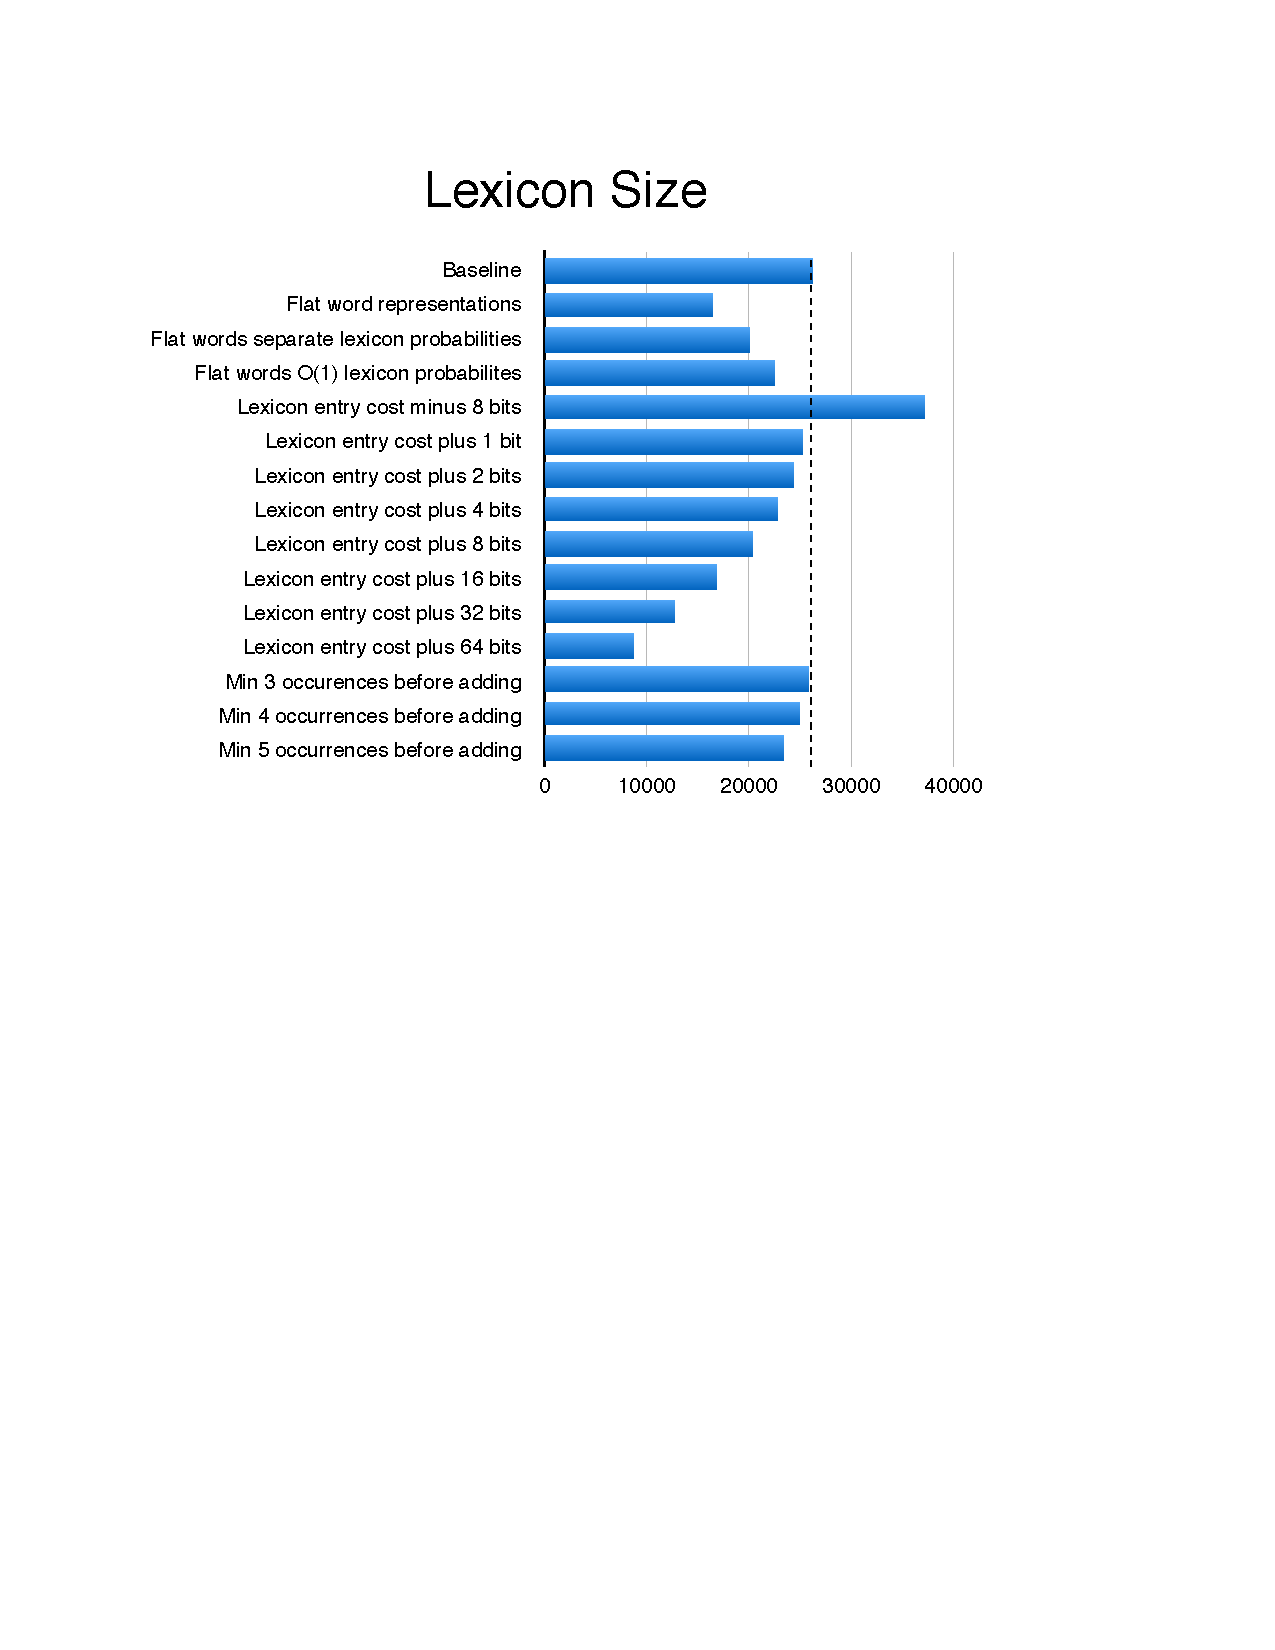
\includegraphics{./figure/lexicon_size.pdf}
  \end{figure}

  De Marcken reports 2.33 bits per character, however our result is 2.23 bits per character. As shown below, after 15 iterations, our algorithm comes to converges. From this perspective, it shows somehow our implementation is correct. But we also notice our range of turblulence is bigger than De Marcken's after 15 iterations.

  \begin{figure}[h]
  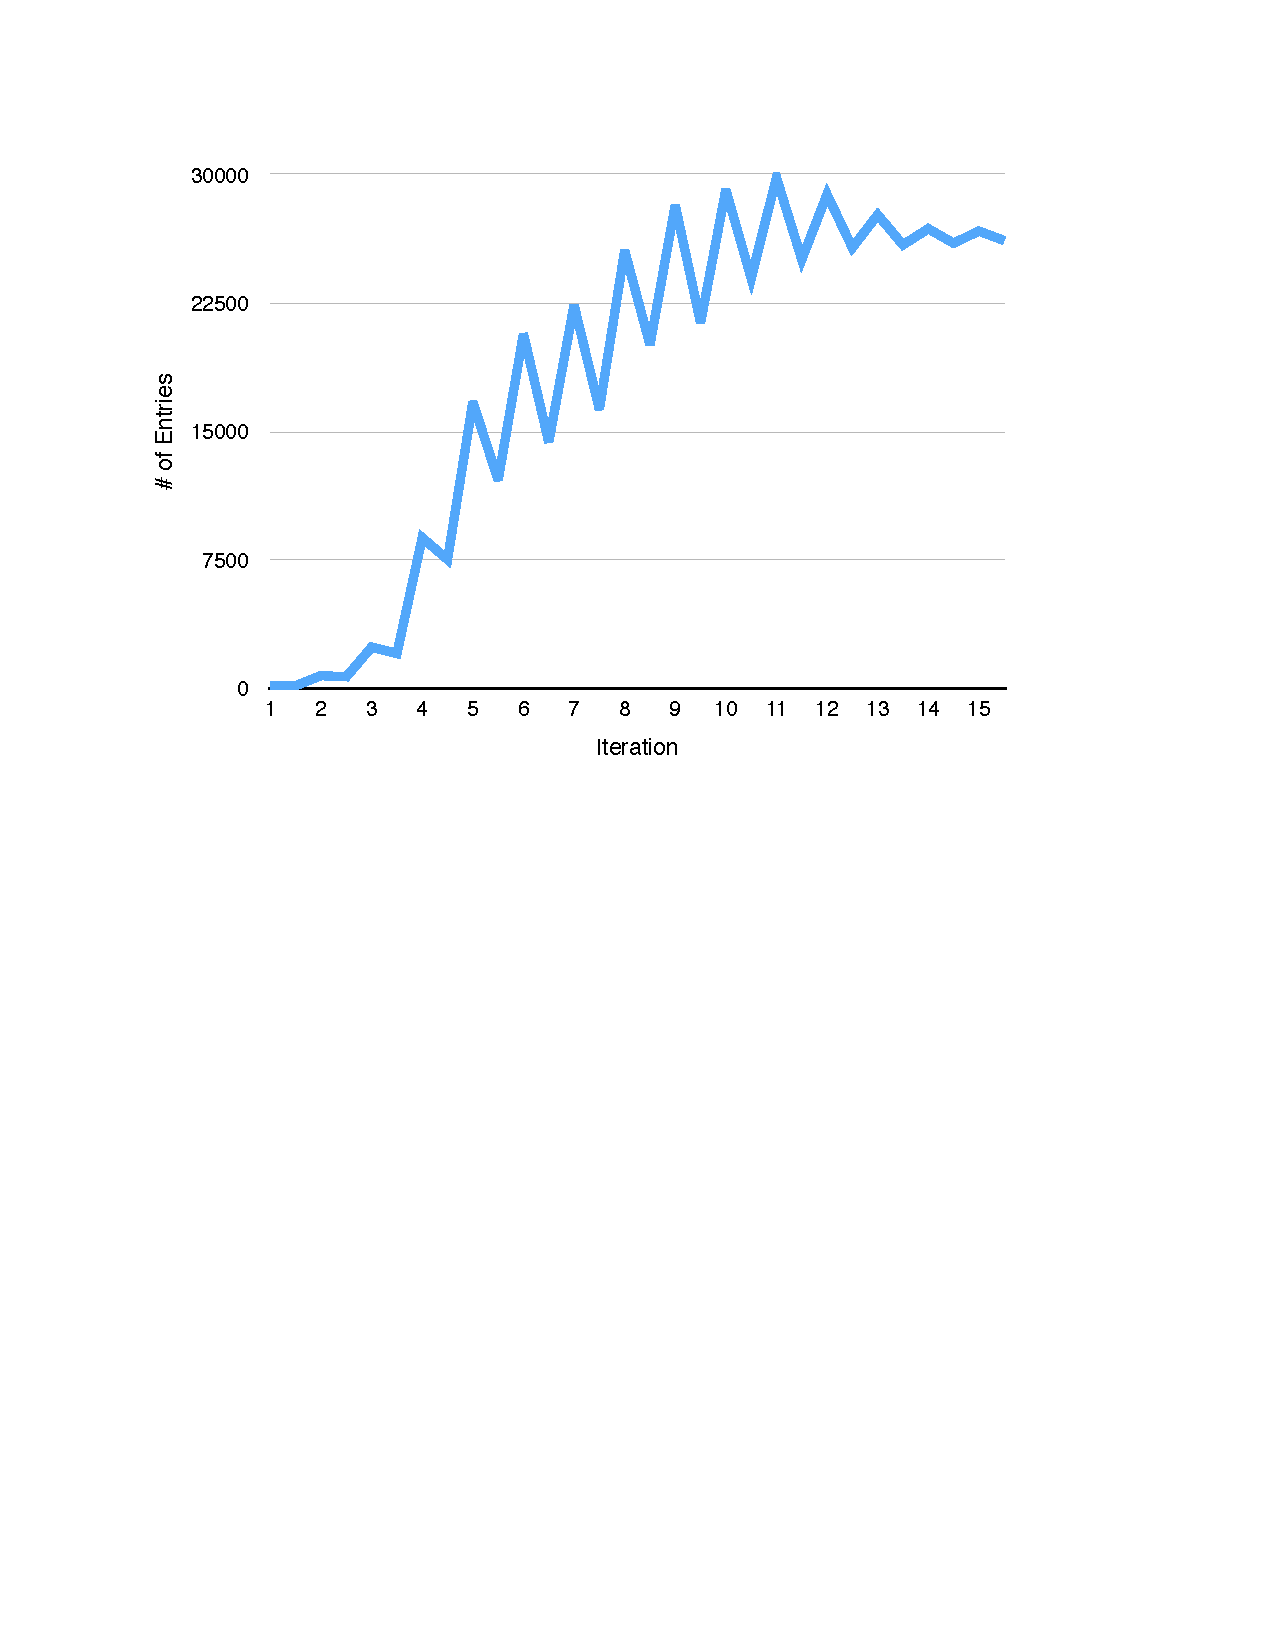
\includegraphics{./figure/entropy_per_iteration.pdf}
  \end{figure}

  Also ,we plot the relation between bits per character and iterations. The more iterations it runs, the smaller the bits per charachter.Similarly, after 15 iterators, the bits per character goes down smoothly. It indicates our algorithm converges. 
  \begin{figure}[h]
  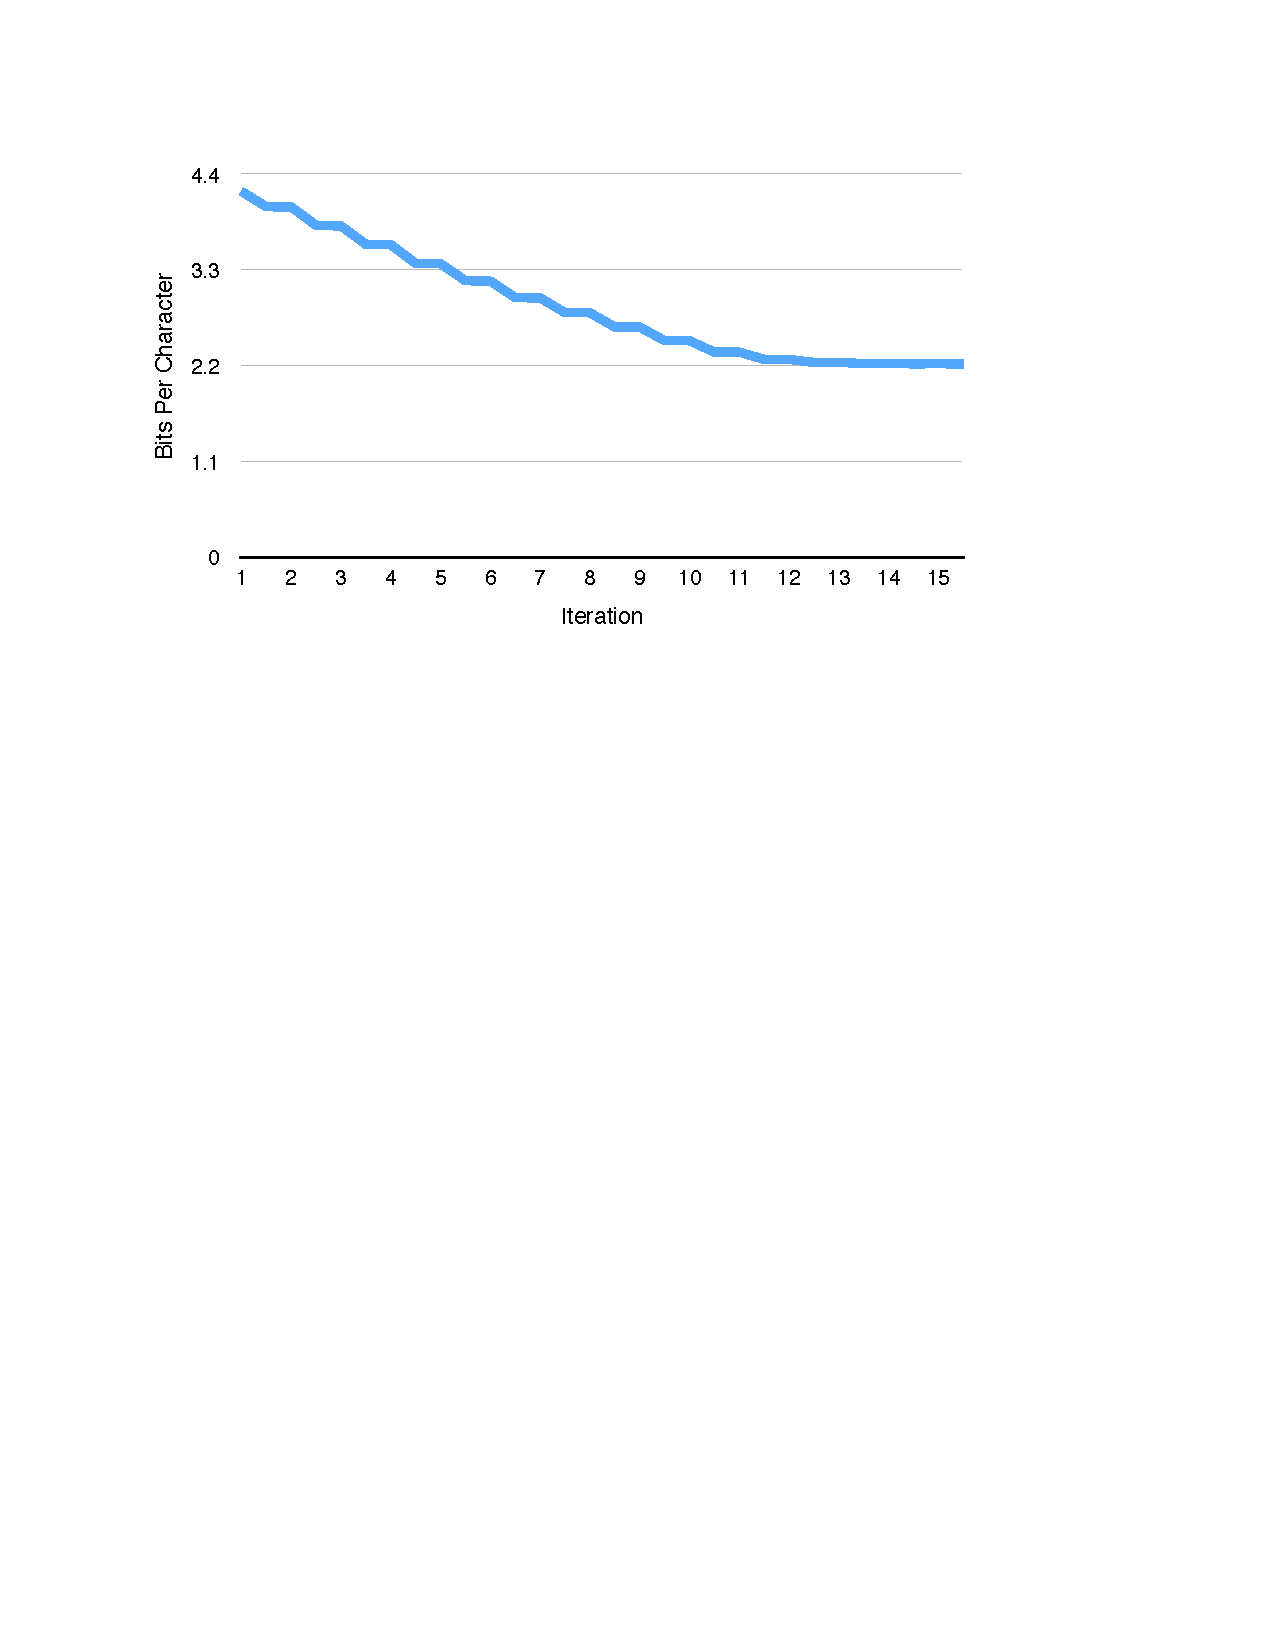
\includegraphics{./figure/bit_of_char_per_iteration.pdf}
  \end{figure}

  During our baseline running, 60\% of found word are exactly correct, 40\% are incorrect. We investigate these incorrect found words deep, and try to categorize what kind error types they belong to. As you can see below, about 43\% of those words combines two true word together as one segmented word, 18\% is our tool find this word but doesn't split it at correct ending character, the error about finding this word but not splitting it at correct starting character also takes almost 18\%. 8.7\% is caused by combining three real words together as one word, while 1.6\% comes from quad+ words combination. We also notice that 6.2\% is for a true word, our tool splits it into several fragements. Sometimes, our tool would find a word, but adding suffix and prefix from its neighbor words, taking 3.3\%.

  \begin{figure}[h]
  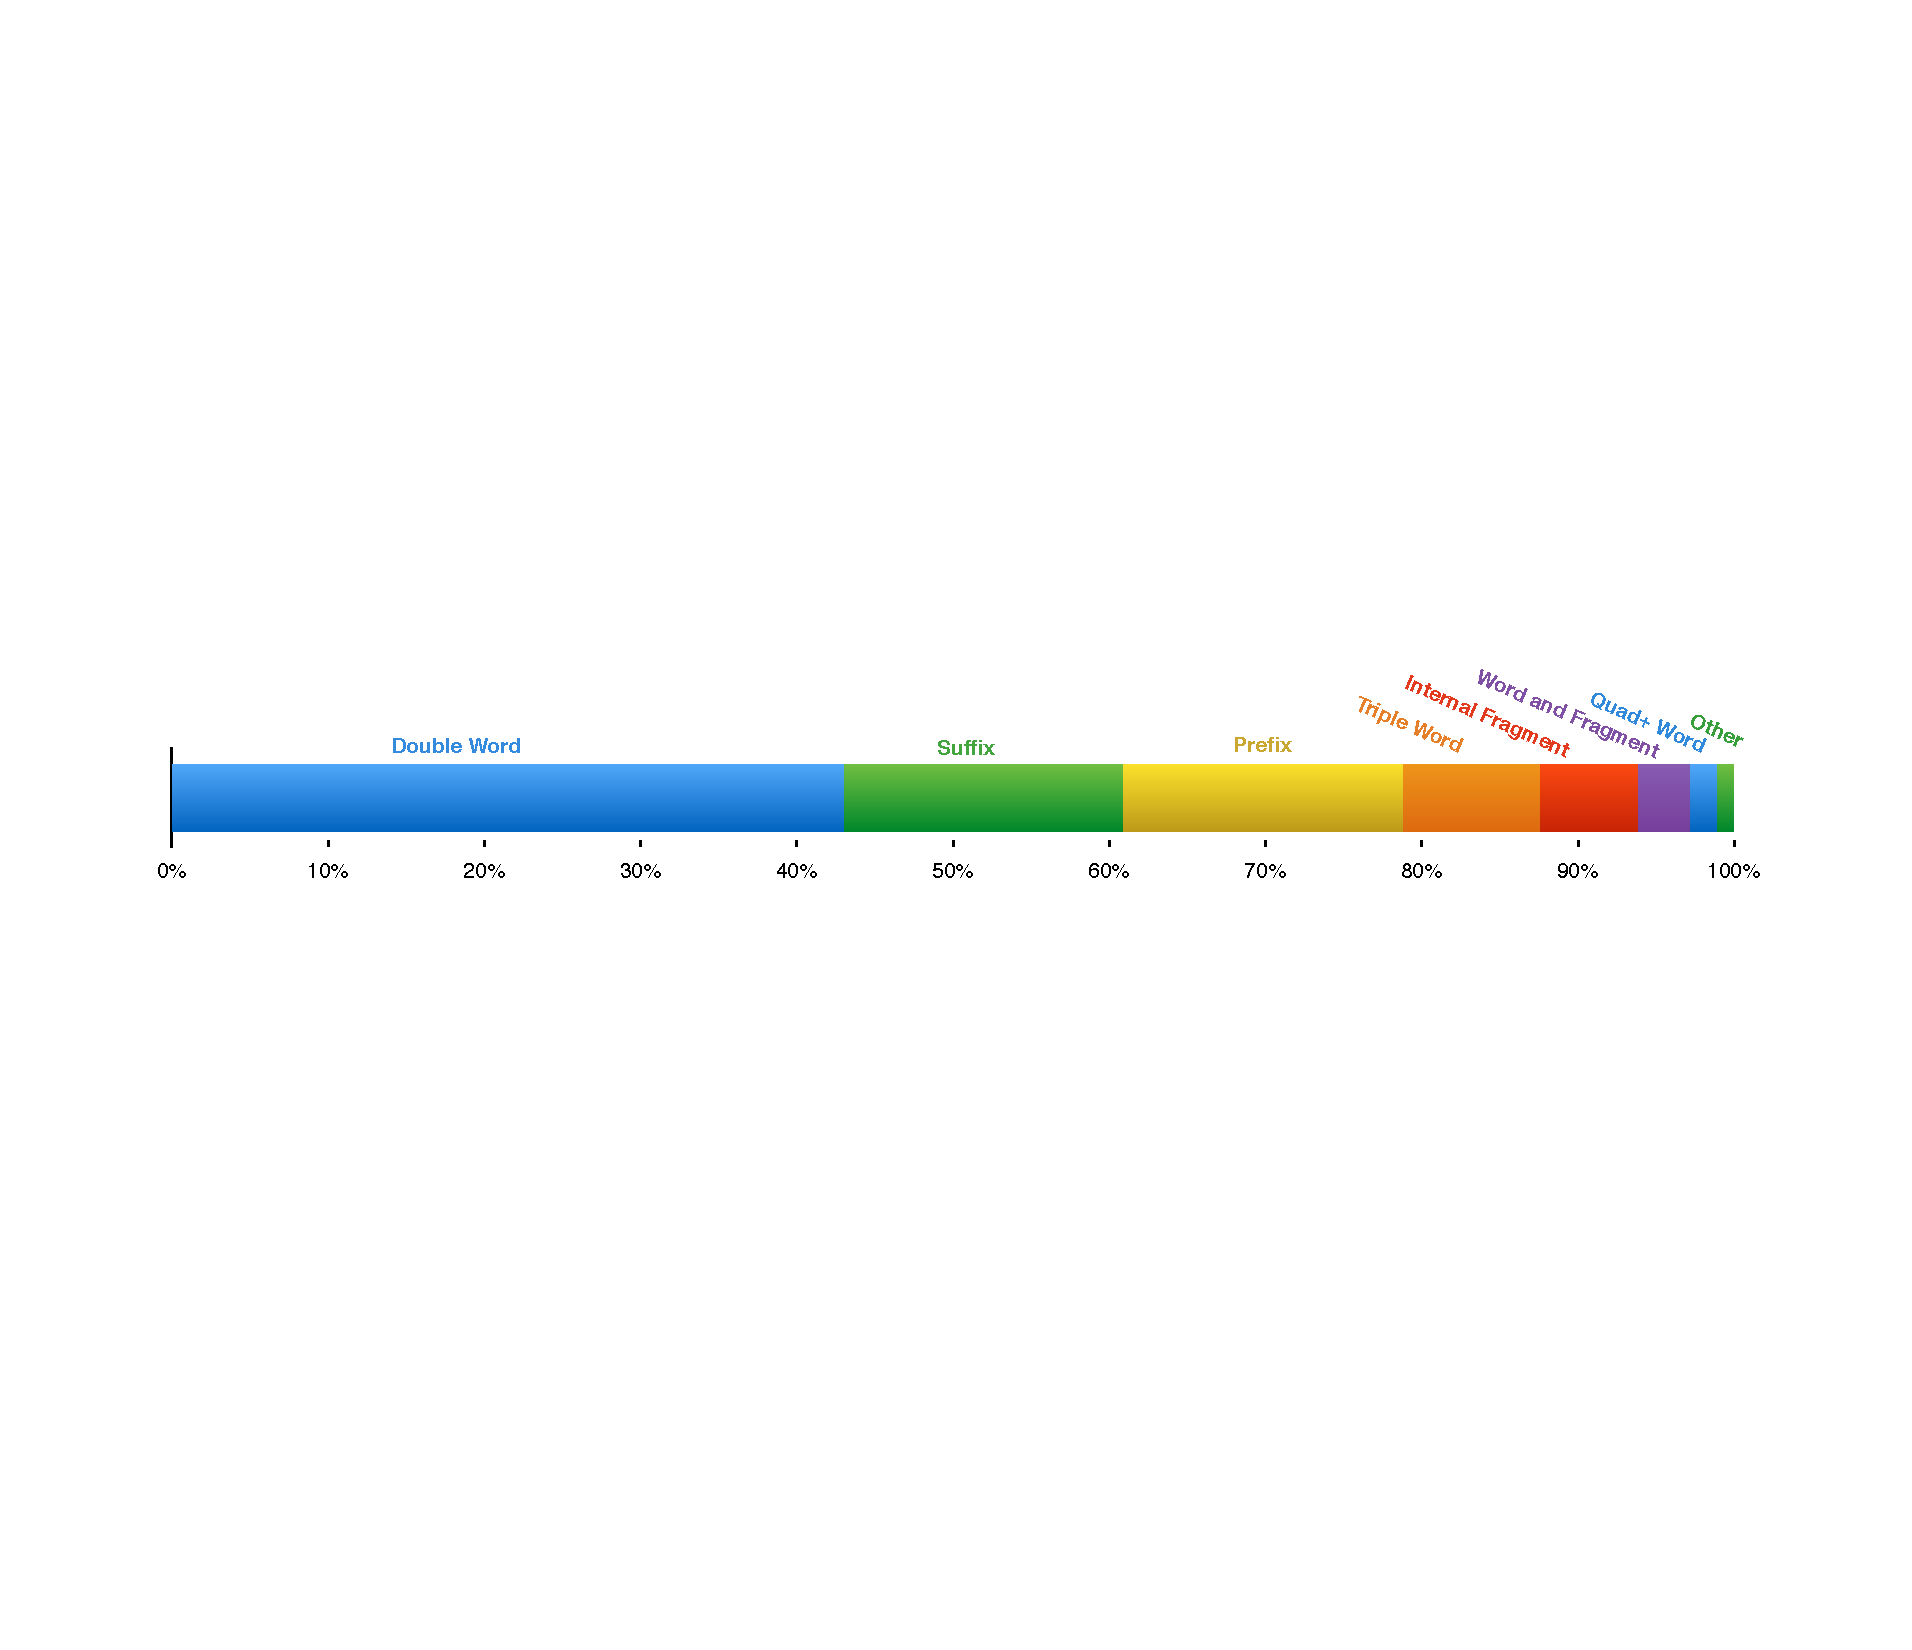
\includegraphics[scale=0.6]{./figure/error_nature_classfier.pdf}
  \end{figure}
  
  \begin{figure}[h]
  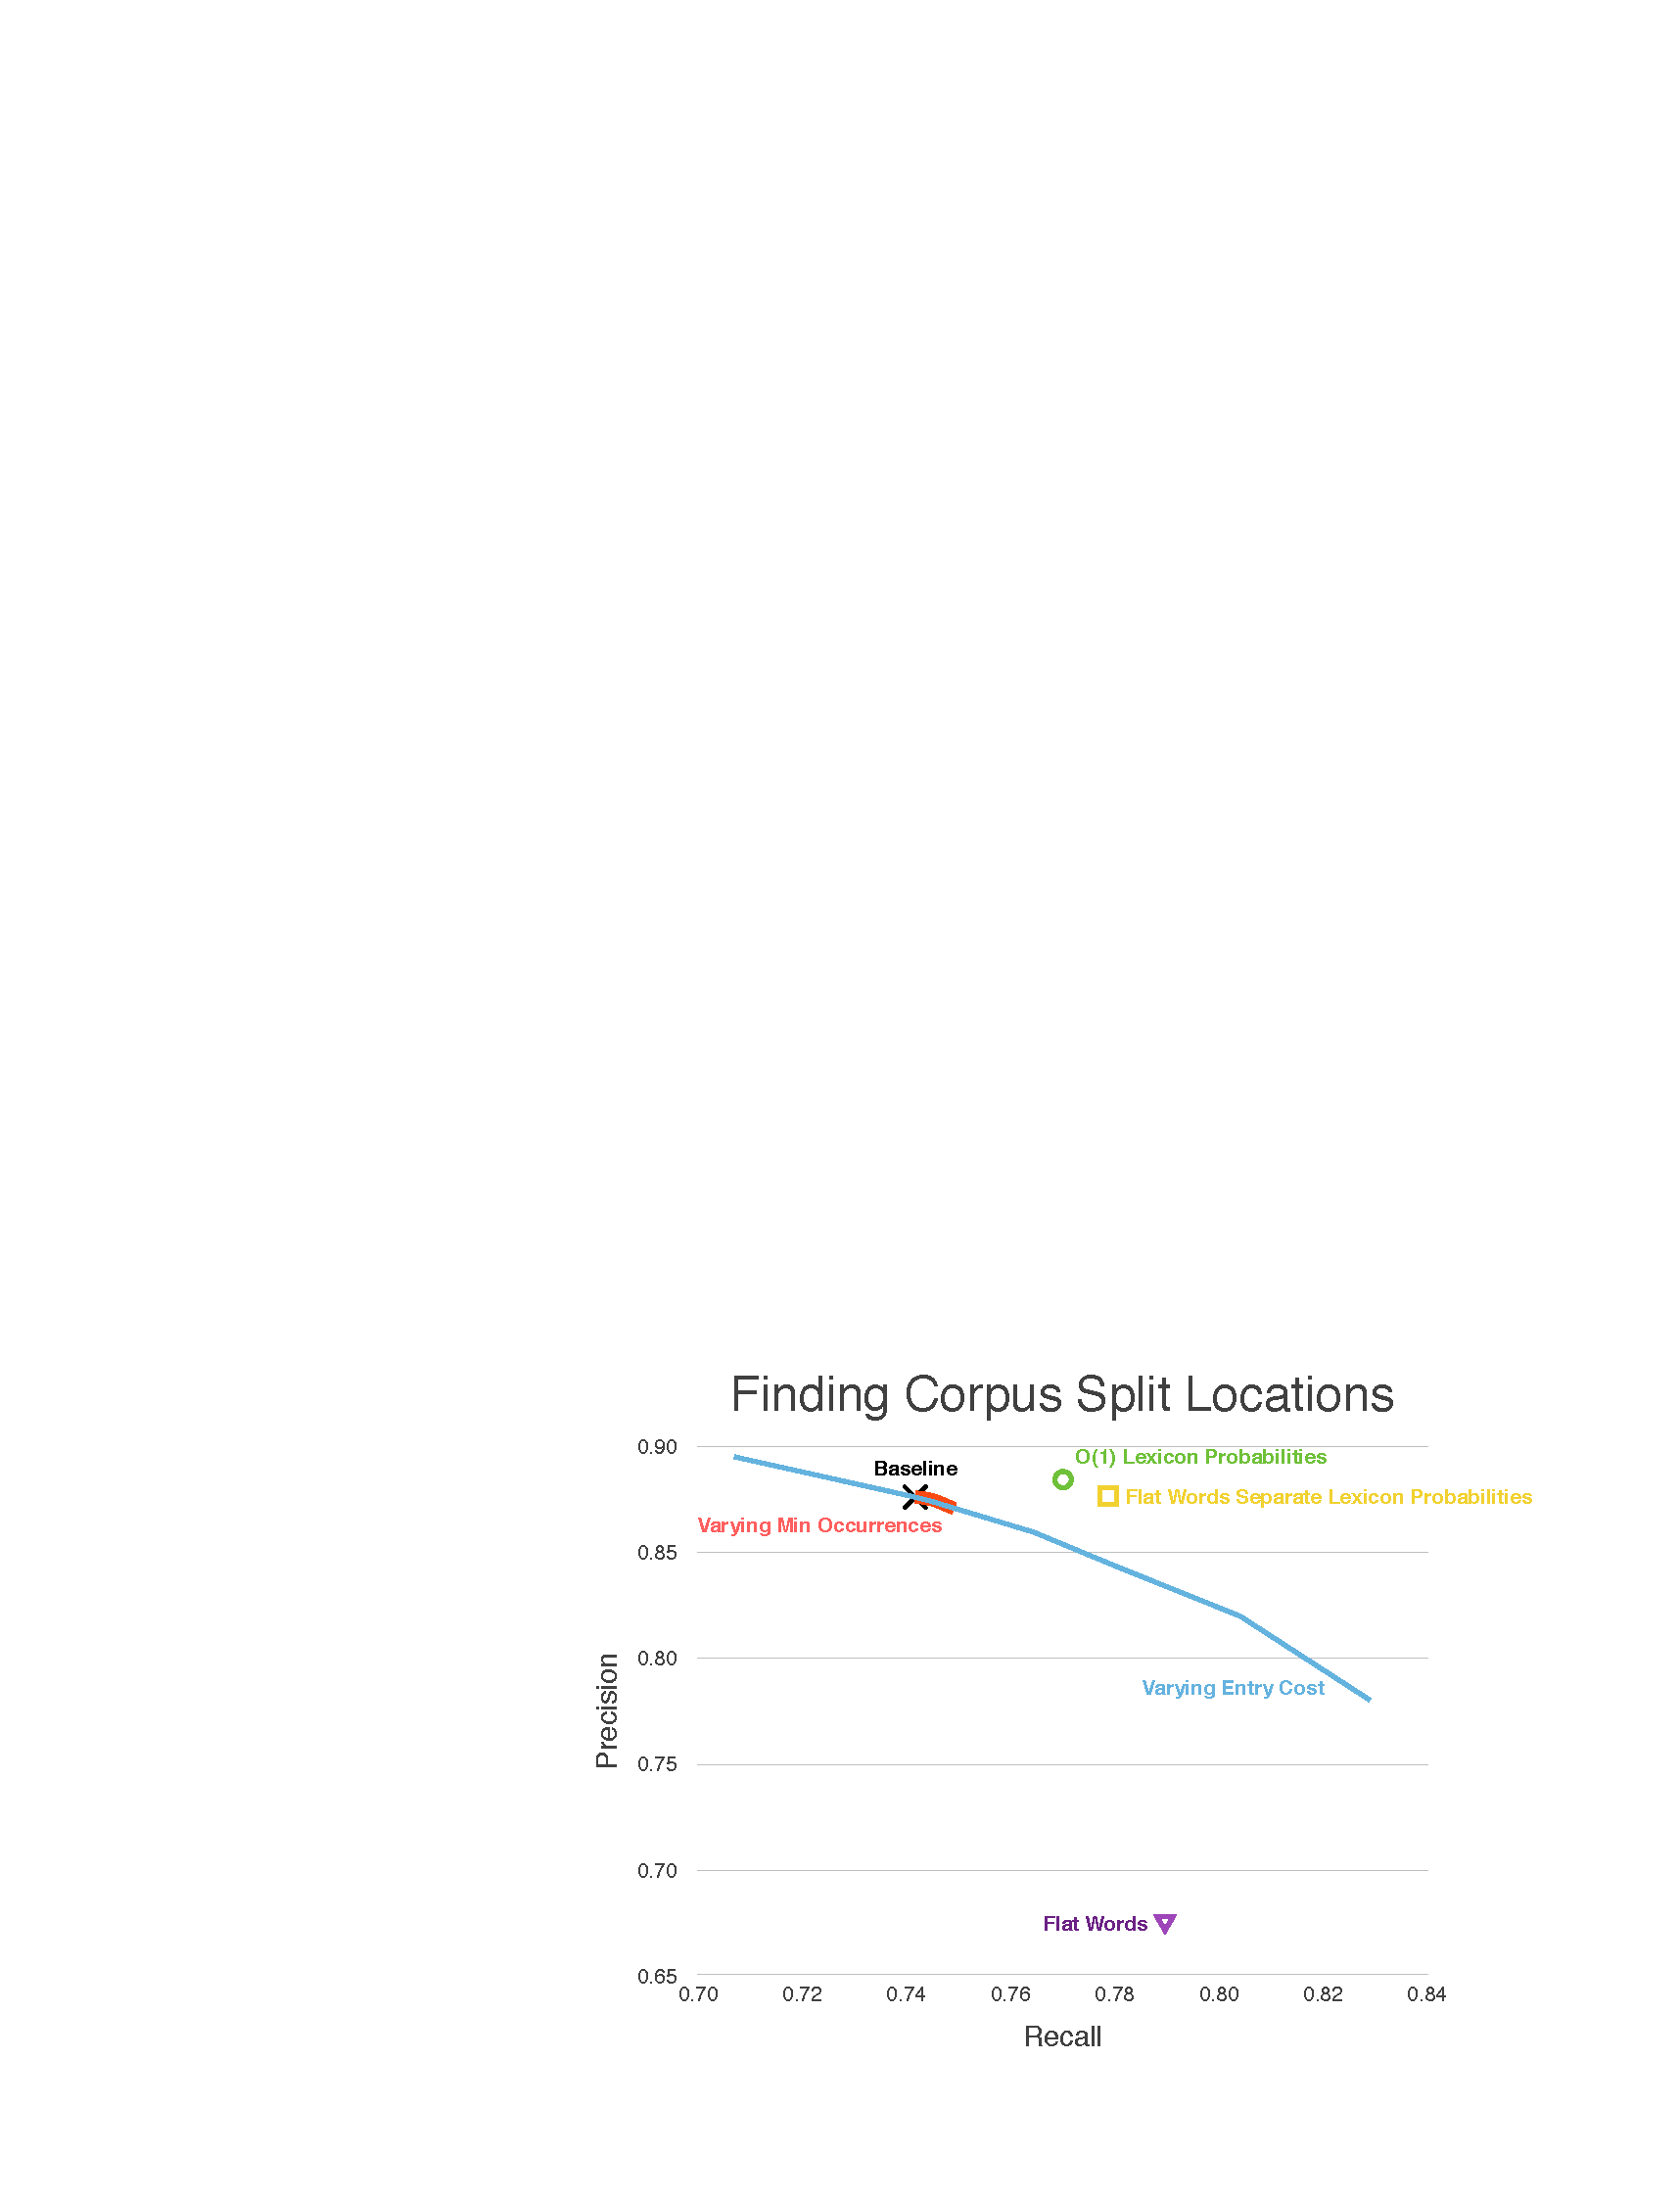
\includegraphics{./figure/finding_corpus_split_location.pdf}
  \end{figure}

  \begin{figure}[h]
  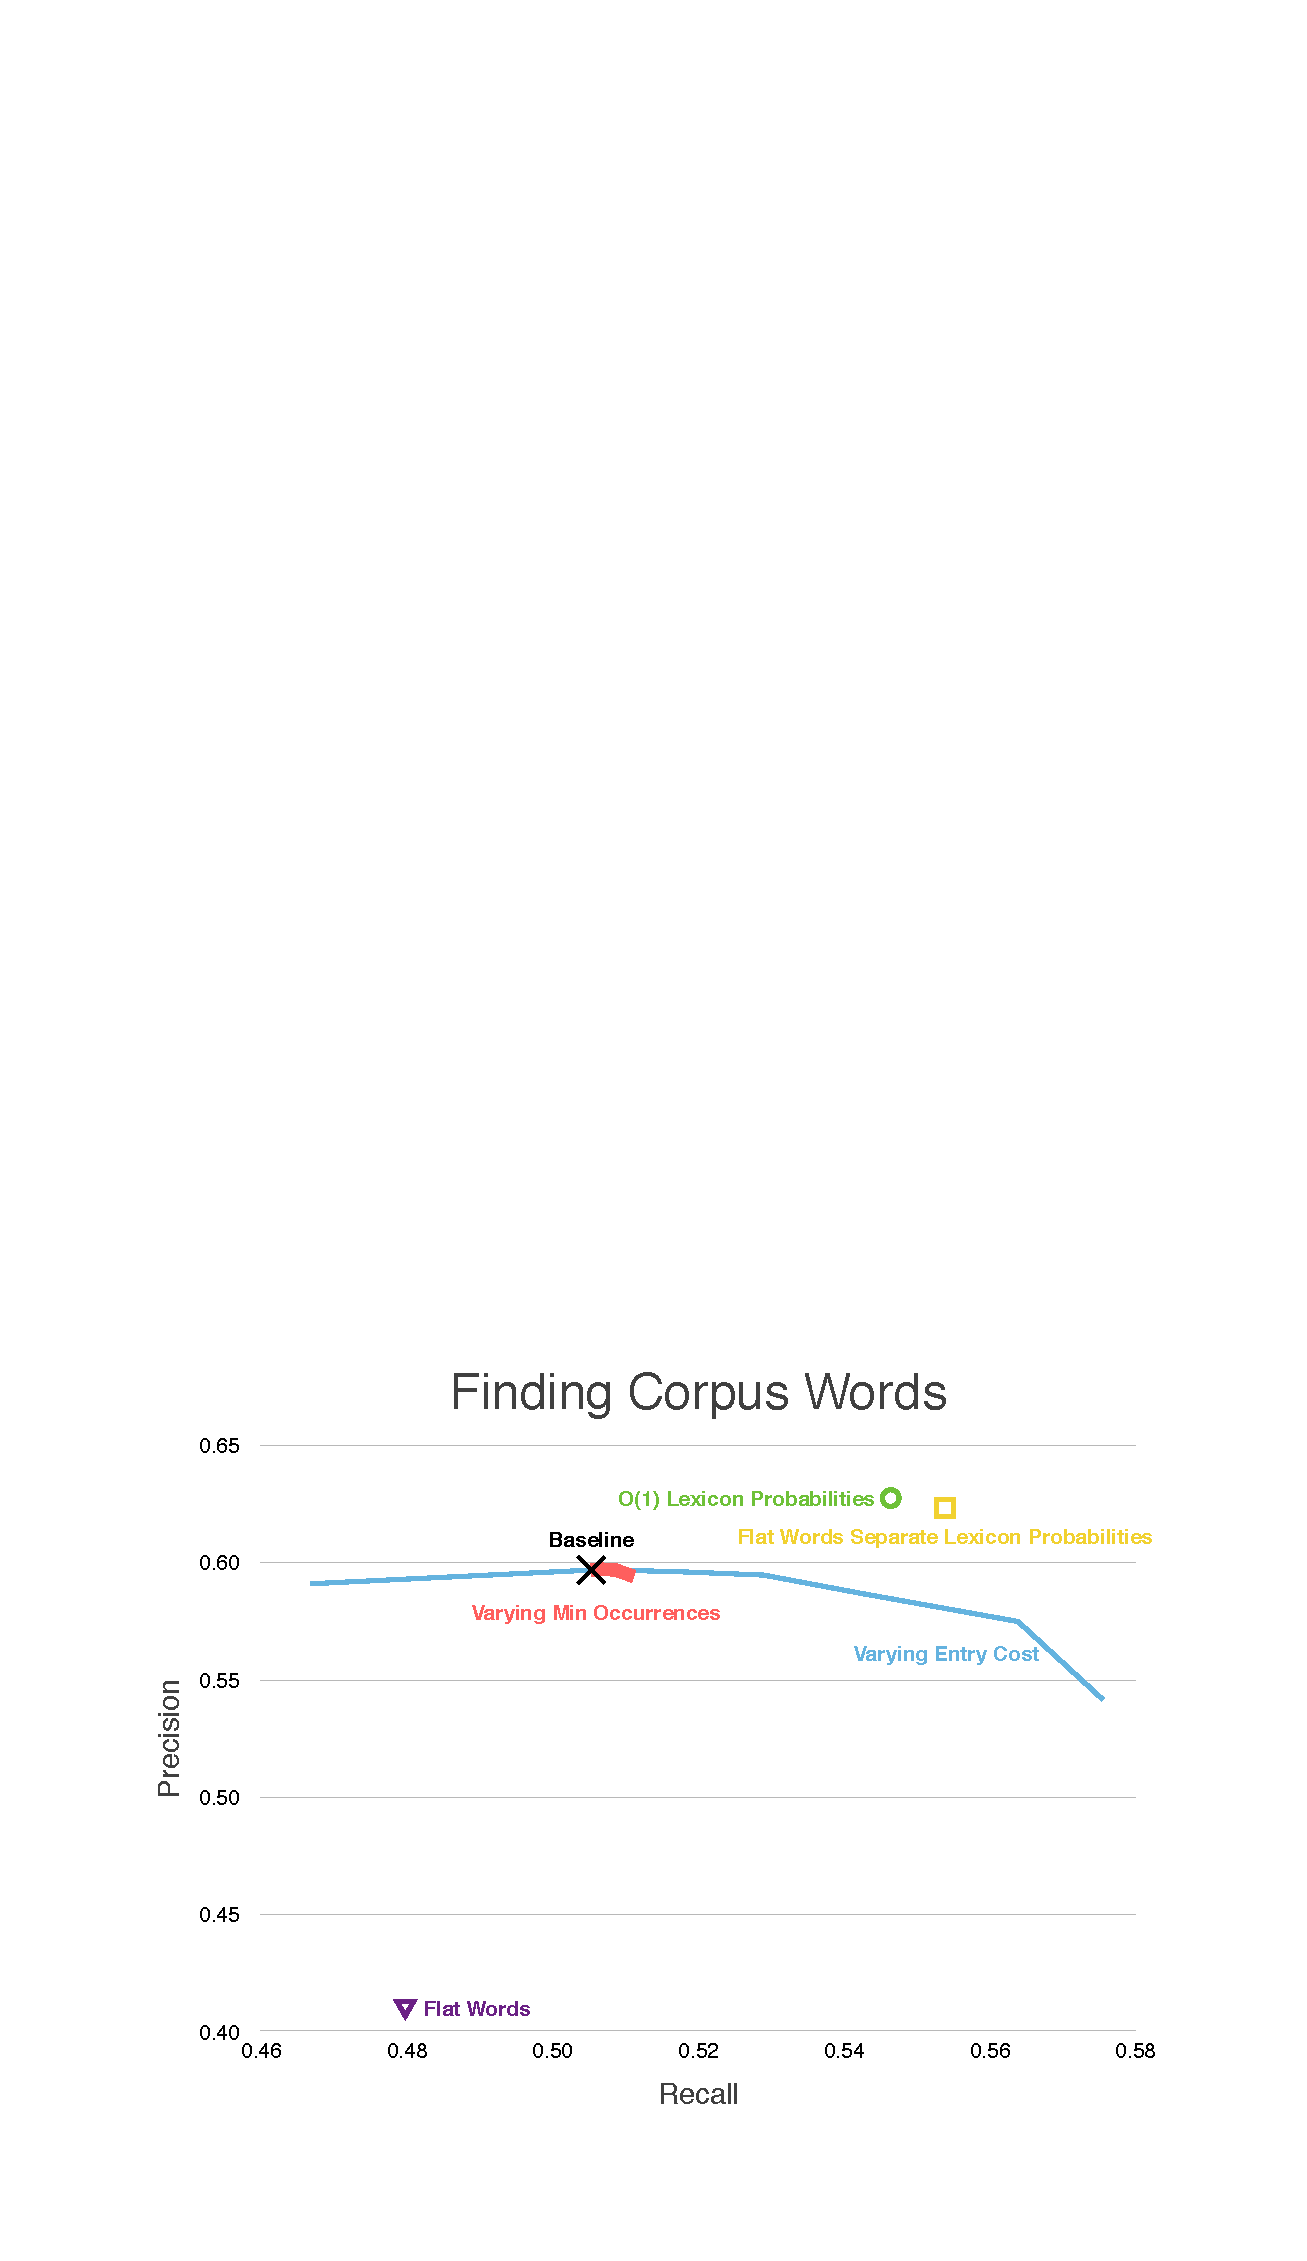
\includegraphics{./figure/finding_corpus_word.pdf}
  \end{figure}

  \begin{figure}[h]
  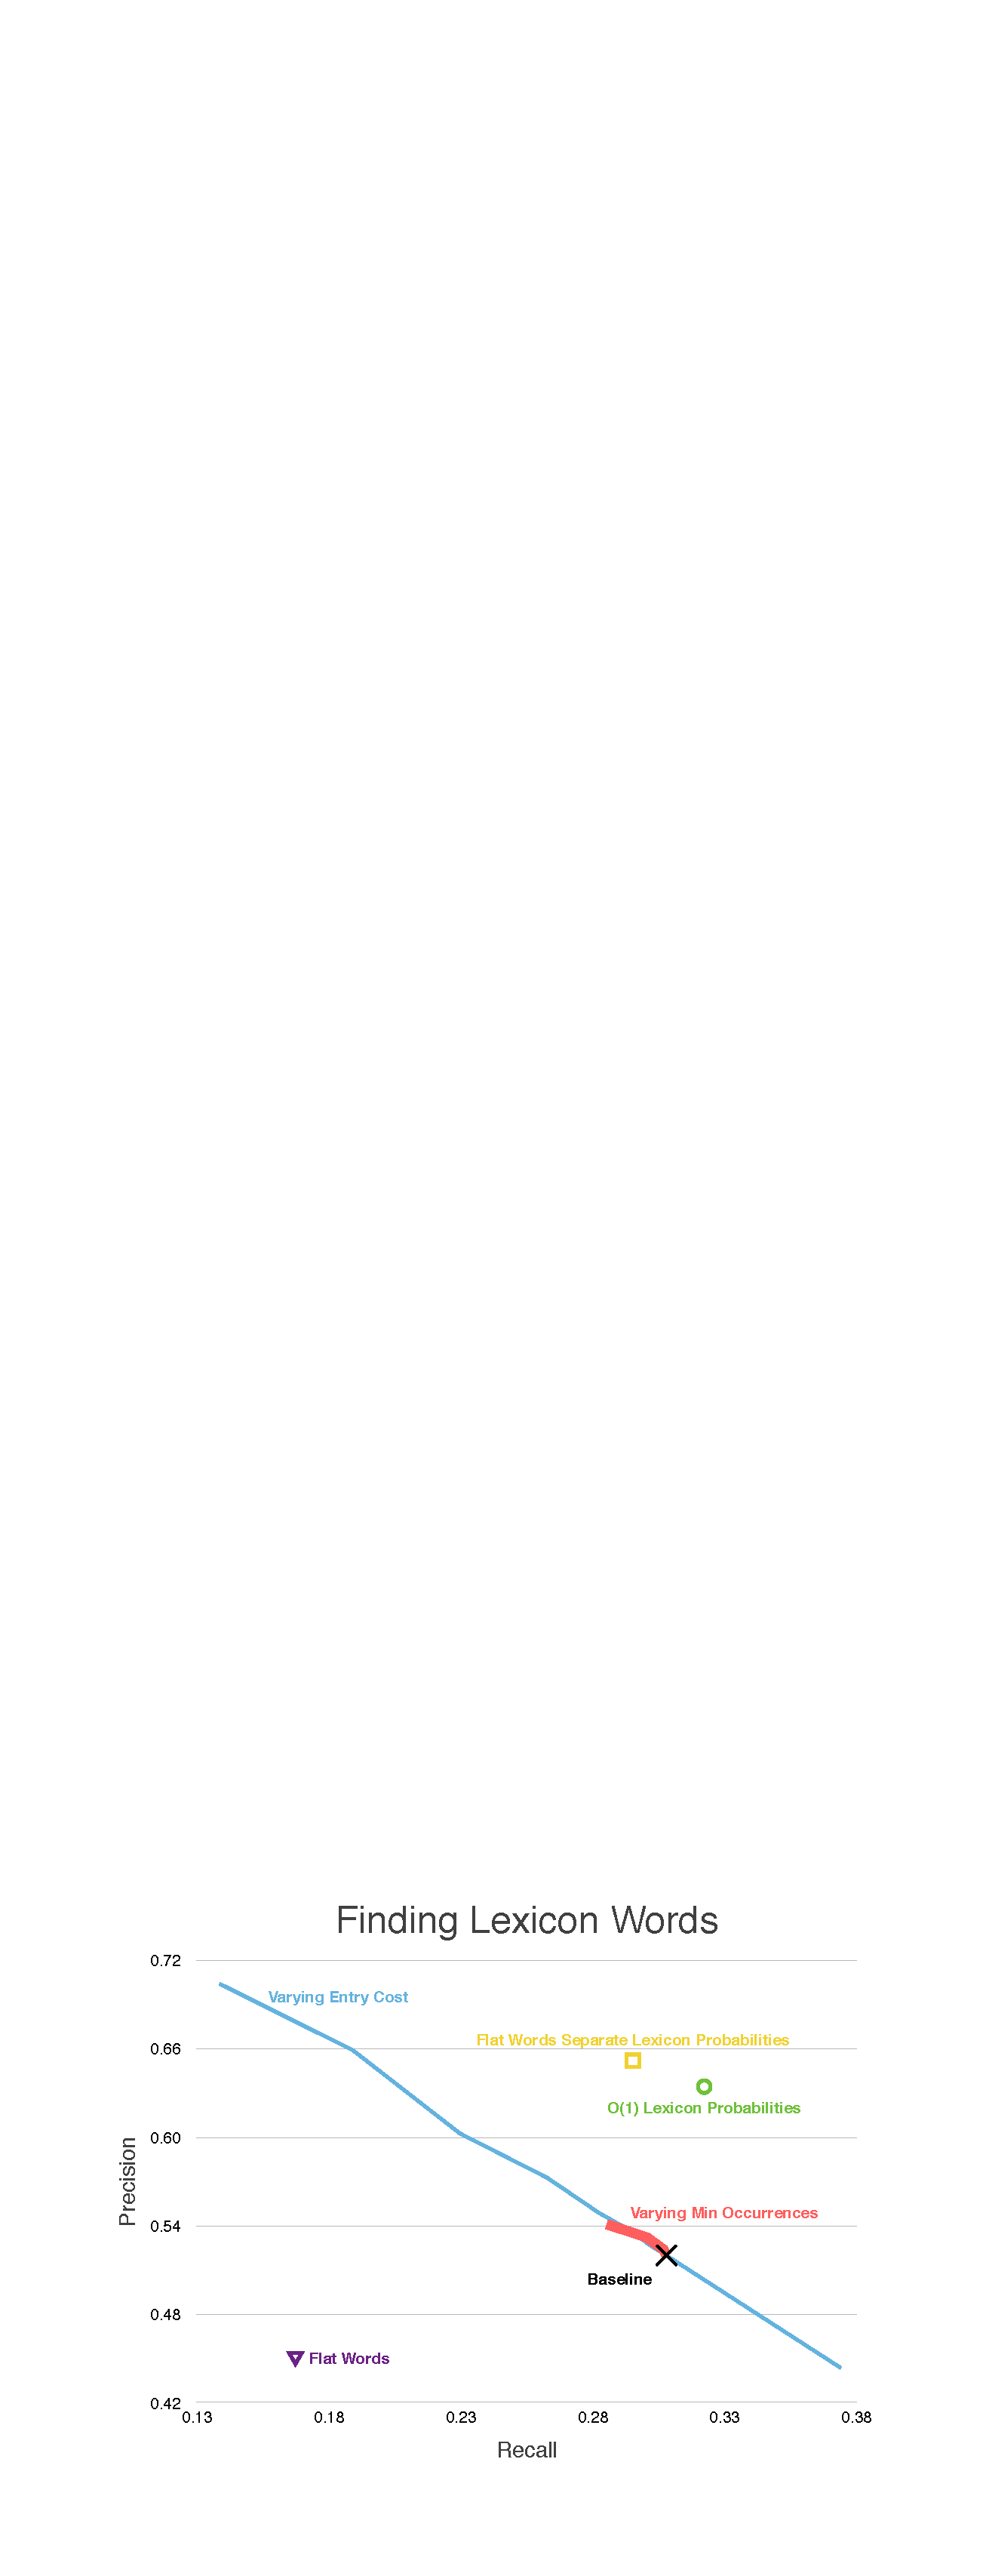
\includegraphics{./figure/finding_lexiocn_words.pdf}
  \end{figure}

  \section{Discussion}

  what do the results mean

  \section{Ideas for Improvement}

  ideas for improvement

\end{document}
